% This is samplepaper.tex, a sample chapter demonstrating the
% LLNCS macro package for Springer Computer Science proceedings;
% Version 2.20 of 2017/10/04
%
\documentclass[runningheads]{llncs}
%
\usepackage{graphicx}
% Used for displaying a sample figure. If possible, figure files should
% be included in EPS format.
%
% If you use the hyperref package, please uncomment the following line
% to display URLs in blue roman font according to Springer's eBook style:
% \renewcommand\UrlFont{\color{blue}\rmfamily}

\begin{document}
%
\title{Programming Assignment 1 Solution}
\author{Fahim Tahmid Chowdhury}
\institute{Florida State University}
\maketitle              % typeset the header of the contribution
%

\section{Support Vector Machine (SVM)}
\subsection{Answer to 1(a)}
The soft margin classification algorithm is implemented in the \texttt{svm\_model.py} file of the submitted code.

\subsection{Answer to 1(b)}
The random dataset is generated according to the project specification while keeping the random seed fixed to 33290.
The dataset generation is implemented in \texttt{generate\_random\_data.py}.
The dataset is fed to the SVM model and the value of C is varied from 1000.1, 100.1, 0.001 to 0.0001.
\figurename~\ref{fig:svm_c_1000.1}, \figurename~\ref{fig:svm_c_100.1}, \figurename~\ref{fig:svm_c_0.001} and
\figurename~\ref{fig:svm_c_0.0001} depict the results for SVM model when C = 1000.1, 100.1, 0.001 and 0.0001, respectively.
All the figures show the datapoints, i.e. red crosses and green crosses belong to Class A and B respectively,
the support vectors are circles by blue circles. The classifier is denoted by the solid black line and the decision boundaries are shown by the
dashed lines.
The misclassification error, leave-one-out cross validation error and margin for different values of C are mentioned in Table~\ref{tab:table_C}.
For the dataset generated, we get 

\begin{table}
\caption{SVM results on Dummy Dataset for different values of C}\label{tab:table_C}
\begin{tabular}{|l|l|l|l|}
\hline
C &  Misclassification Error & Leave-one-out Cross Validation Error & Margin\\
\hline
1000.1 & 0.0825 & 0.0825 & 0.4736146883359073\\
100.1 & 0.085 & 0.085 & 0.473277758987939\\
0.001 & 0.085 & 0.085 & 2.4963754697373535\\
0.0001 & 0.0875 & 0.0875 & 17.677670988643605\\
\hline
\end{tabular}
\end{table}

\begin{figure}
\centering
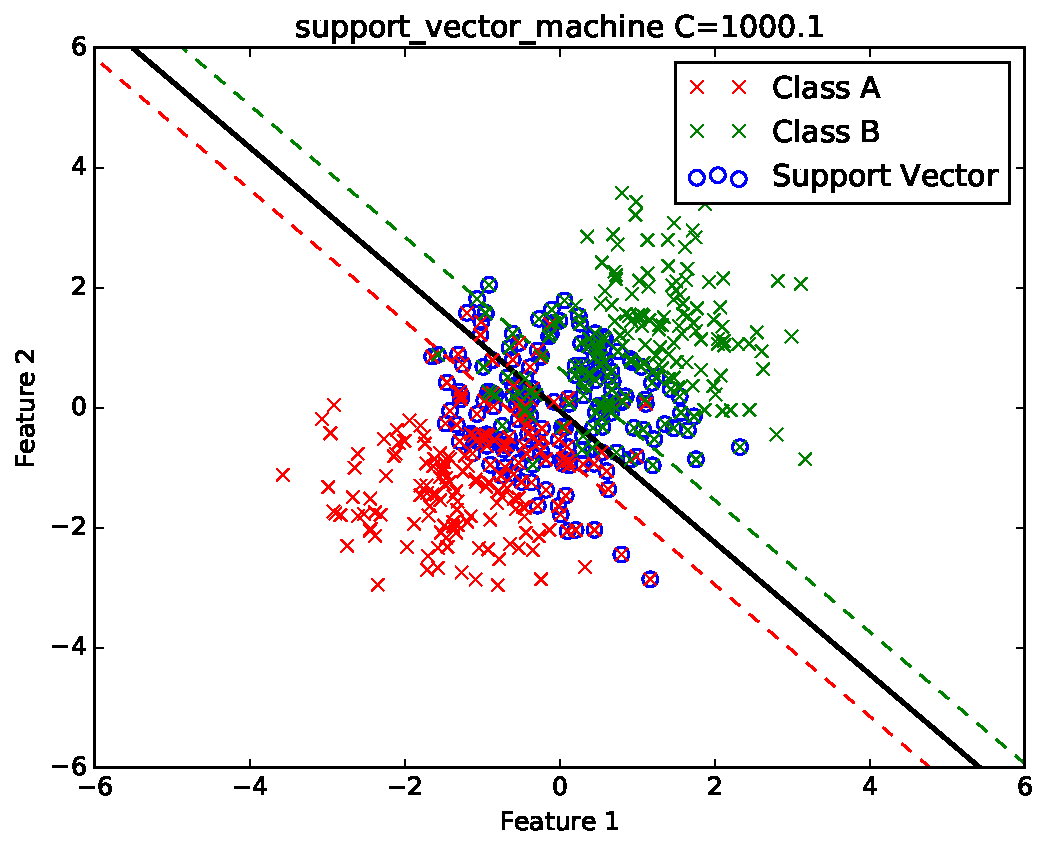
\includegraphics[width=0.75\textwidth]{support_vector_machine1000_1.pdf}
\caption{SVM model for C=1000.1} \label{fig:svm_c_1000.1}
\end{figure}
\begin{figure}
\centering
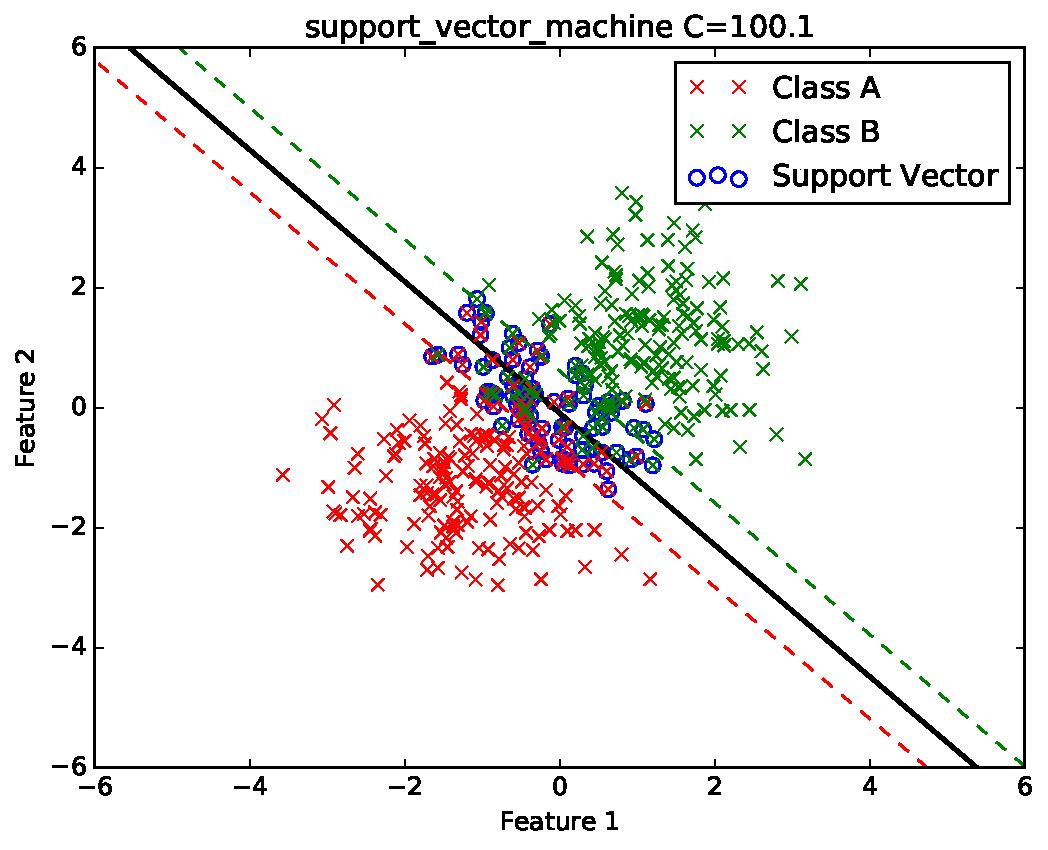
\includegraphics[width=0.75\textwidth]{support_vector_machine100_1.pdf}
\caption{SVM model for C=100.1} \label{fig:svm_c_100.1}
\end{figure}
\begin{figure}
\centering
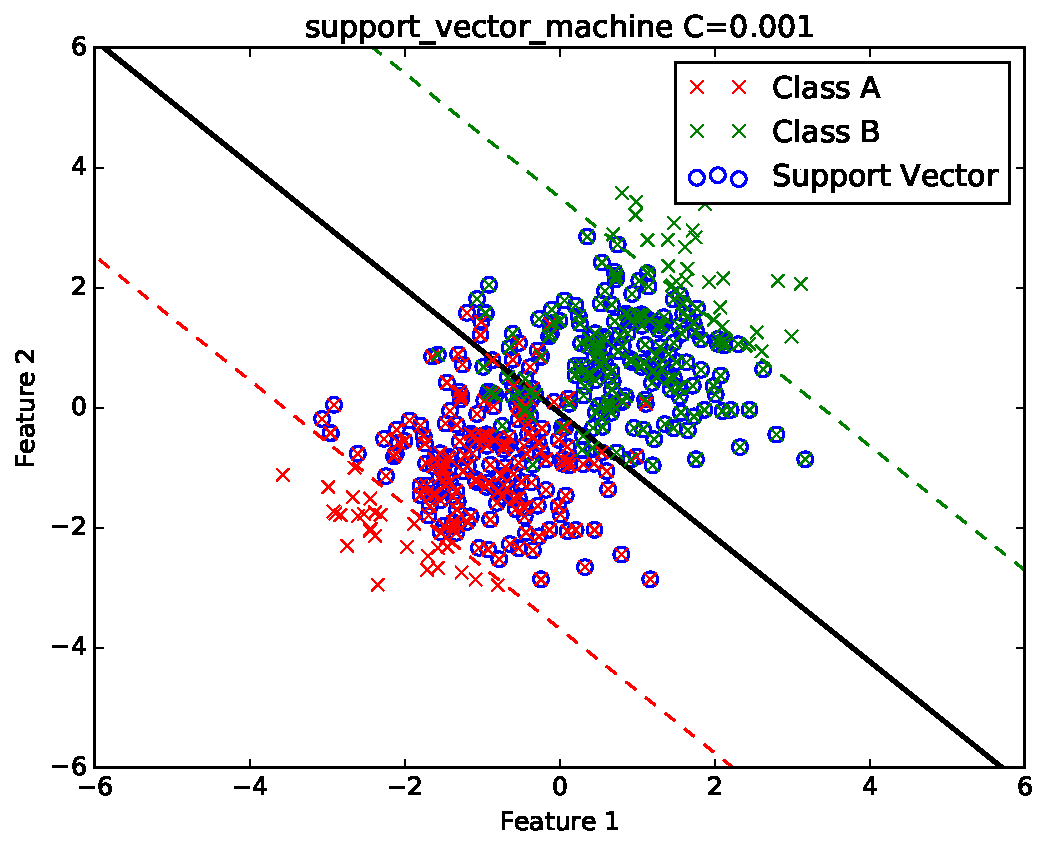
\includegraphics[width=0.75\textwidth]{support_vector_machine0_001.pdf}
\caption{SVM model for C=0.001} \label{fig:svm_c_0.001}
\end{figure}
\begin{figure}
\centering
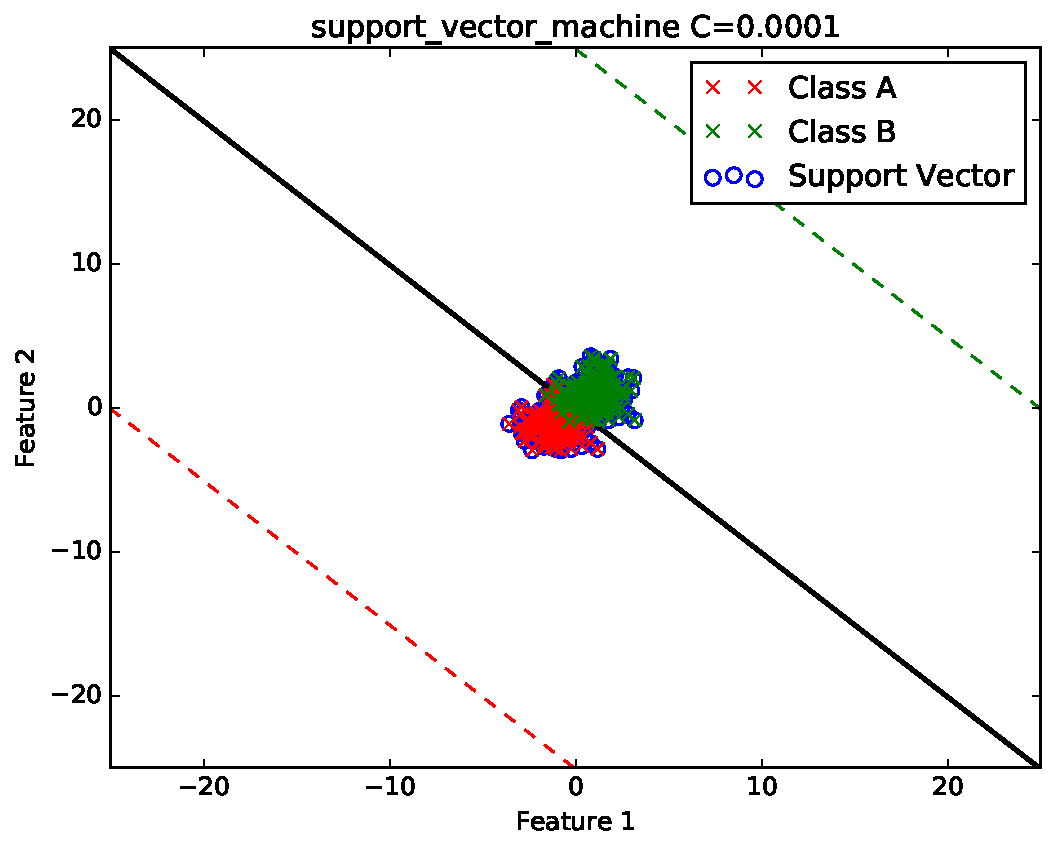
\includegraphics[width=0.75\textwidth]{support_vector_machine0_0001.pdf}
\caption{SVM model for C=0.0001} \label{fig:svm_c_0.0001}
\end{figure}

\subsection{Answer to 1(c)}
Only the samples with 0 and 1 labels in the MNIST dataset are filtered out in \texttt{mnist\_reader.py} file.
For training the SVM model with MNIST, the value for the tradeoff variable C is set to 1000.1.
The Generalization Error is 0.0009456264775413711 in this case.

\end{document}
